%%%%%%%%%%%%%%%%%%%%%%%%%%%%%%%%%%%%%%%%%%%%%%%%%%%%%%%%%%%%%%%%%%%%%%%%%%%%%%%%%%
\begin{frame}[fragile]\frametitle{}
\begin{center}
{\Large Different Large Language Models}

\end{center}
\end{frame}

%%%%%%%%%%%%%%%%%%%%%%%%%%%%%%%%%%%%%%%%%%%%%%%%%%%%%%%%%%%
\begin{frame}[fragile]\frametitle{Transformer Models}



		\begin{center}
		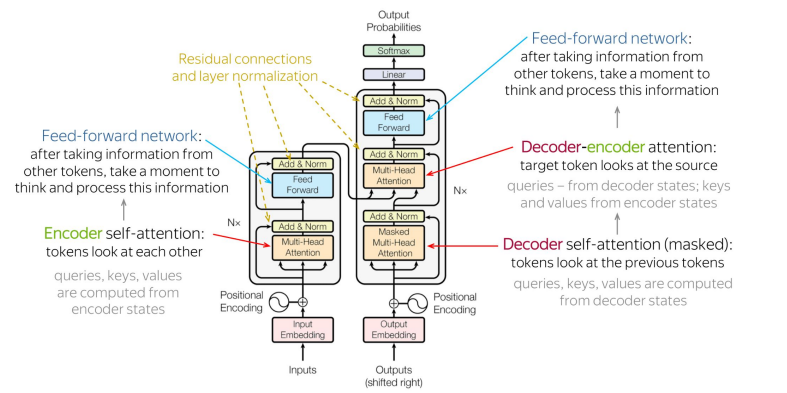
\includegraphics[width=\linewidth,keepaspectratio]{promptengg81}

		{\tiny (Ref: The Complete Prompt Engineering for AI Bootcamp (2023))}
		\end{center}	

\end{frame}



%%%%%%%%%%%%%%%%%%%%%%%%%%%%%%%%%%%%%%%%%%%%%%%%%%%%%%%%%%%
\begin{frame}[fragile]\frametitle{GPT3}


\begin{columns}
    \begin{column}[T]{0.6\linewidth}
		\begin{center}
		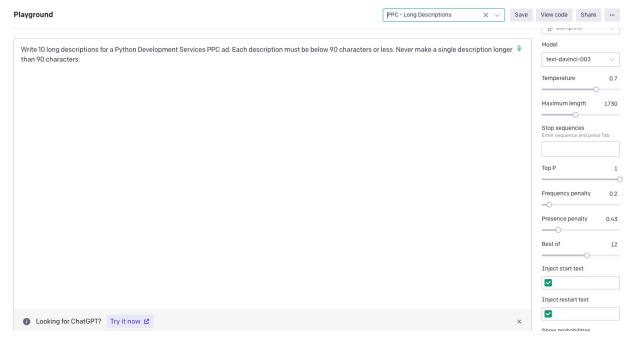
\includegraphics[width=\linewidth,keepaspectratio]{promptengg82}

		{\tiny (Ref: The Complete Prompt Engineering for AI Bootcamp (2023))}
		\end{center}	
    \end{column}
    \begin{column}[T]{0.4\linewidth}
		Created by OpenAI
		Access it with code or without (Playground https://platform.openai.com/playground)
    \end{column}
  \end{columns}
\end{frame}

%%%%%%%%%%%%%%%%%%%%%%%%%%%%%%%%%%%%%%%%%%%%%%%%%%%%%%%%%%%
\begin{frame}[fragile]\frametitle{GPT3 Features}


		\begin{center}
		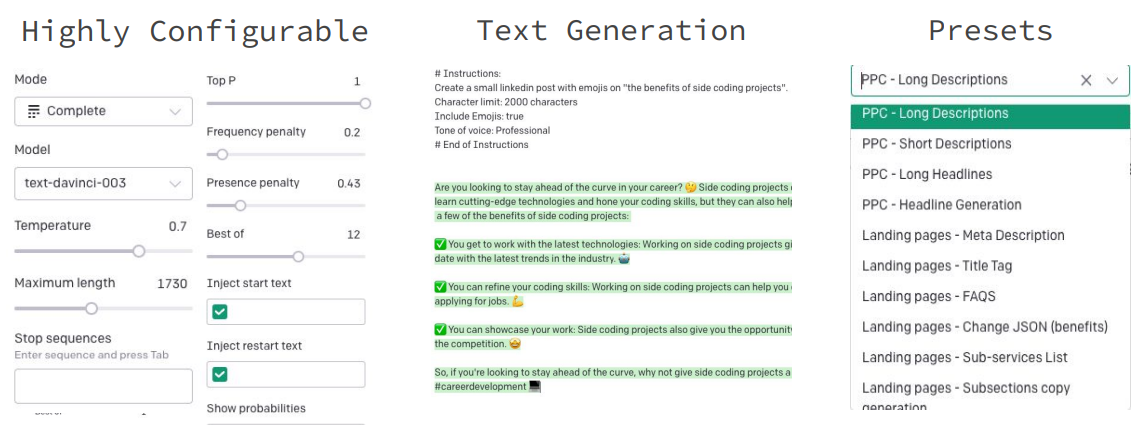
\includegraphics[width=\linewidth,keepaspectratio]{promptengg83}

		{\tiny (Ref: The Complete Prompt Engineering for AI Bootcamp (2023))}
		\end{center}	

\end{frame}


%%%%%%%%%%%%%%%%%%%%%%%%%%%%%%%%%%%%%%%%%%%%%%%%%%%%%%%%%%%
\begin{frame}[fragile]\frametitle{GPT3 Usecases}


		\begin{center}
		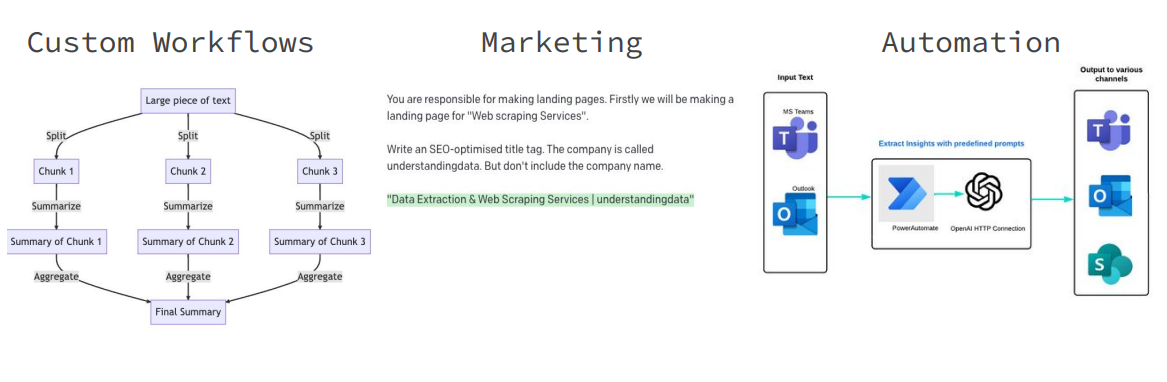
\includegraphics[width=\linewidth,keepaspectratio]{promptengg84}

		{\tiny (Ref: The Complete Prompt Engineering for AI Bootcamp (2023))}
		\end{center}	

\end{frame}

%%%%%%%%%%%%%%%%%%%%%%%%%%%%%%%%%%%%%%%%%%%%%%%%%%%%%%%%%%%
\begin{frame}[fragile]\frametitle{GPT3 Limitations}




\begin{itemize}
\item  Unlike ChatGPT, GPT-3 doesn’t store chat history, which can lead to you needing to re-inject the extra context into the
original prompt.
\item Tokens are currently limited to 4000 tokens per output. This includes both your initial prompt the text generated
from ChatGPT.

\end{itemize}	 

{\tiny (Ref: The Complete Prompt Engineering for AI Bootcamp (2023))}

\end{frame}


%%%%%%%%%%%%%%%%%%%%%%%%%%%%%%%%%%%%%%%%%%%%%%%%%%%%%%%%%%%
\begin{frame}[fragile]\frametitle{Bard}


\begin{columns}
    \begin{column}[T]{0.6\linewidth}
		\begin{center}
		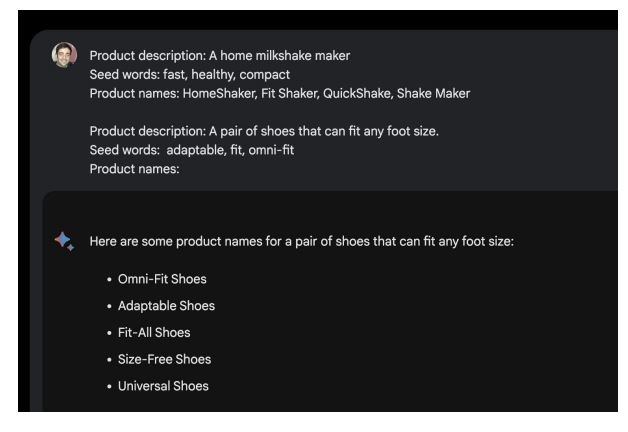
\includegraphics[width=\linewidth,keepaspectratio]{promptengg85}

		{\tiny (Ref: The Complete Prompt Engineering for AI Bootcamp (2023))}
		\end{center}	
    \end{column}
    \begin{column}[T]{0.4\linewidth}
		Created by Google
		Access it via chat https://bard.google.com/ or encounter it in search results
    \end{column}
  \end{columns}
\end{frame}

%%%%%%%%%%%%%%%%%%%%%%%%%%%%%%%%%%%%%%%%%%%%%%%%%%%%%%%%%%%
\begin{frame}[fragile]\frametitle{Bard Features}


		\begin{center}
		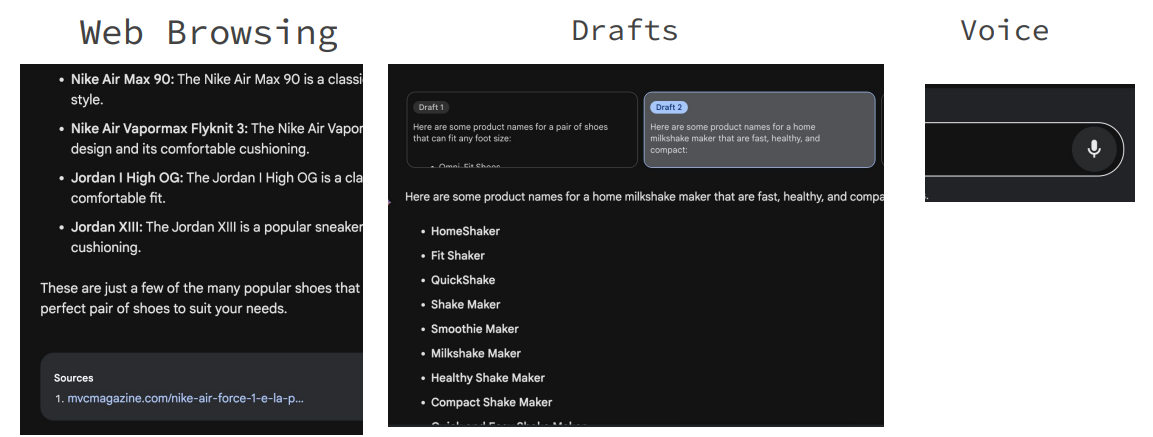
\includegraphics[width=\linewidth,keepaspectratio]{promptengg86}

		{\tiny (Ref: The Complete Prompt Engineering for AI Bootcamp (2023))}
		\end{center}	

\end{frame}

%%%%%%%%%%%%%%%%%%%%%%%%%%%%%%%%%%%%%%%%%%%%%%%%%%%%%%%%%%%
\begin{frame}[fragile]\frametitle{Bard Usecases}


		\begin{center}
		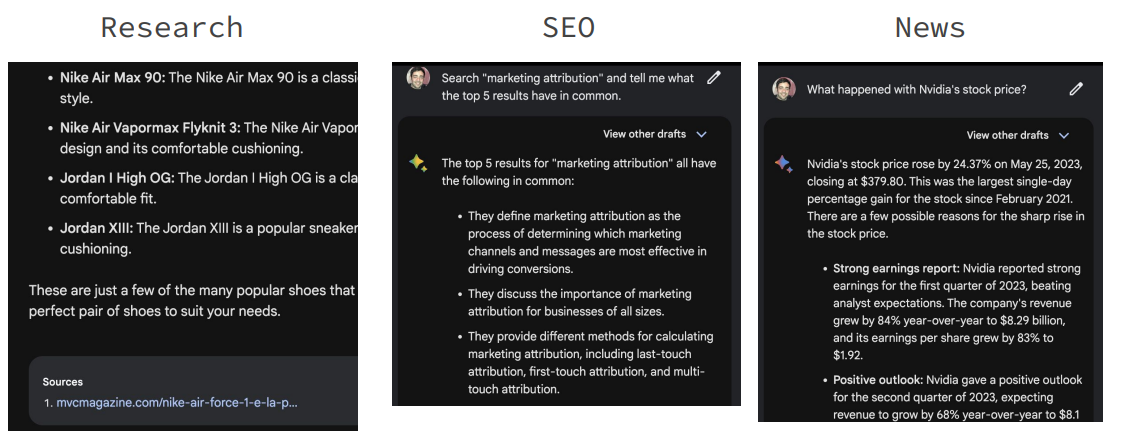
\includegraphics[width=\linewidth,keepaspectratio]{promptengg87}

		{\tiny (Ref: The Complete Prompt Engineering for AI Bootcamp (2023))}
		\end{center}	

\end{frame}



%%%%%%%%%%%%%%%%%%%%%%%%%%%%%%%%%%%%%%%%%%%%%%%%%%%%%%%%%%%
\begin{frame}[fragile]\frametitle{Meta LLaMA}


\begin{columns}
    \begin{column}[T]{0.6\linewidth}
		\begin{center}
		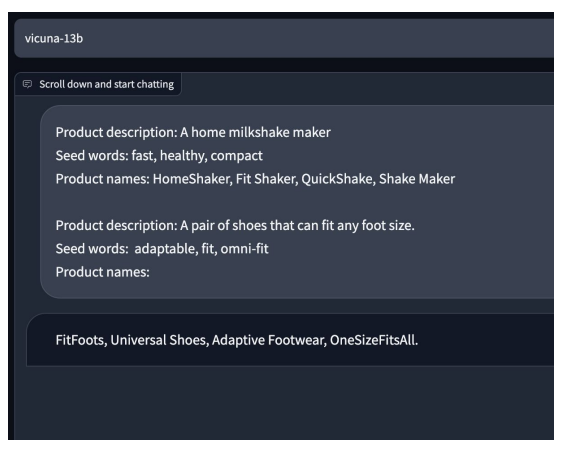
\includegraphics[width=\linewidth,keepaspectratio]{promptengg88}

		{\tiny (Ref: The Complete Prompt Engineering for AI Bootcamp (2023))}
		\end{center}	
    \end{column}
    \begin{column}[T]{0.4\linewidth}
		Created by Meta and open-sourced / leaked
		Access via hugging face or lmsys https://chat.lmsys.org/
		Use one of the fine-tuned models (i.e. Vicuna) for better results
    \end{column}
  \end{columns}
\end{frame}


%%%%%%%%%%%%%%%%%%%%%%%%%%%%%%%%%%%%%%%%%%%%%%%%%%%%%%%%%%%
\begin{frame}[fragile]\frametitle{Meta LLaMA}

\begin{itemize}
\item  Open-Source. Need to build a UX and any advanced functionality around it, and may need to fine-tune it.
\item Many use-cases in the enterprise can’t use OpenAI for fear of sensitive data leaking or being used to train the model (though OpenAI claims to keep API data private).
\item If you have 200+ examples fine-tuning beats prompt engineering for a specific defined task.
\end{itemize}	 

{\tiny (Ref: The Complete Prompt Engineering for AI Bootcamp (2023))}

\end{frame}

%%%%%%%%%%%%%%%%%%%%%%%%%%%%%%%%%%%%%%%%%%%%%%%%%%%%%%%%%%%
\begin{frame}[fragile]\frametitle{Anthropic Claude}


\begin{columns}
    \begin{column}[T]{0.6\linewidth}
		\begin{center}
		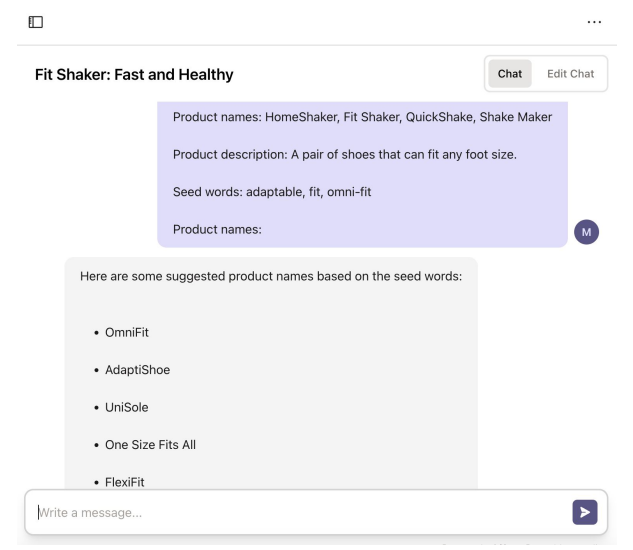
\includegraphics[width=\linewidth,keepaspectratio]{promptengg90}

		{\tiny (Ref: The Complete Prompt Engineering for AI Bootcamp (2023))}
		\end{center}	
    \end{column}
    \begin{column}[T]{0.4\linewidth}
		Created by Anthropic 
		Access via Claude console https://console.anthropic.com/ or API
		Uses Constitutional AI rather than RLHF
    \end{column}
  \end{columns}
\end{frame}

%%%%%%%%%%%%%%%%%%%%%%%%%%%%%%%%%%%%%%%%%%%%%%%%%%%%%%%%%%%
\begin{frame}[fragile]\frametitle{Anthropic Claude Features}


\begin{columns}
    \begin{column}[T]{0.6\linewidth}
		\begin{center}
		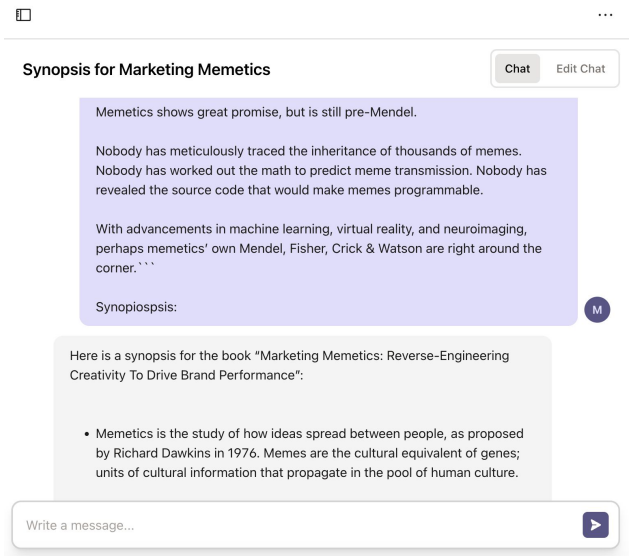
\includegraphics[width=\linewidth,keepaspectratio]{promptengg91}

		{\tiny (Ref: The Complete Prompt Engineering for AI Bootcamp (2023))}
		\end{center}	
    \end{column}
    \begin{column}[T]{0.4\linewidth}
		100k Token Window! 
    \end{column}
  \end{columns}
\end{frame}

%%%%%%%%%%%%%%%%%%%%%%%%%%%%%%%%%%%%%%%%%%%%%%%%%%%%%%%%%%%
\begin{frame}[fragile]\frametitle{Anthropic Claude Use Cases}

\begin{itemize}
\item Large Scale Summarization
\item Book Marketing
\item Writing Styleguides
\end{itemize}	 

{\tiny (Ref: The Complete Prompt Engineering for AI Bootcamp (2023))}

\end{frame}


%%%%%%%%%%%%%%%%%%%%%%%%%%%%%%%%%%%%%%%%%%%%%%%%%%%%%%%%%%%
\begin{frame}[fragile]\frametitle{Microsoft Bing (GPT 4)}


\begin{columns}
    \begin{column}[T]{0.6\linewidth}
		\begin{center}
		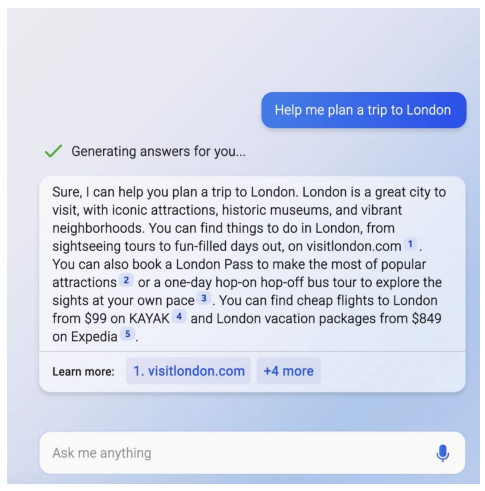
\includegraphics[width=\linewidth,keepaspectratio]{promptengg92}

		{\tiny (Ref: The Complete Prompt Engineering for AI Bootcamp (2023))}
		\end{center}	
    \end{column}
    \begin{column}[T]{0.4\linewidth}
		Powered by OpenAI’s GPT-4
		Access it via chat https://www.microsoft.com/en-gb/bing or encounter it in search results
    \end{column}
  \end{columns}
\end{frame}


%%%%%%%%%%%%%%%%%%%%%%%%%%%%%%%%%%%%%%%%%%%%%%%%%%%%%%%%%%%
\begin{frame}[fragile]\frametitle{Microsoft Bing (GPT 4) Features}


		\begin{center}
		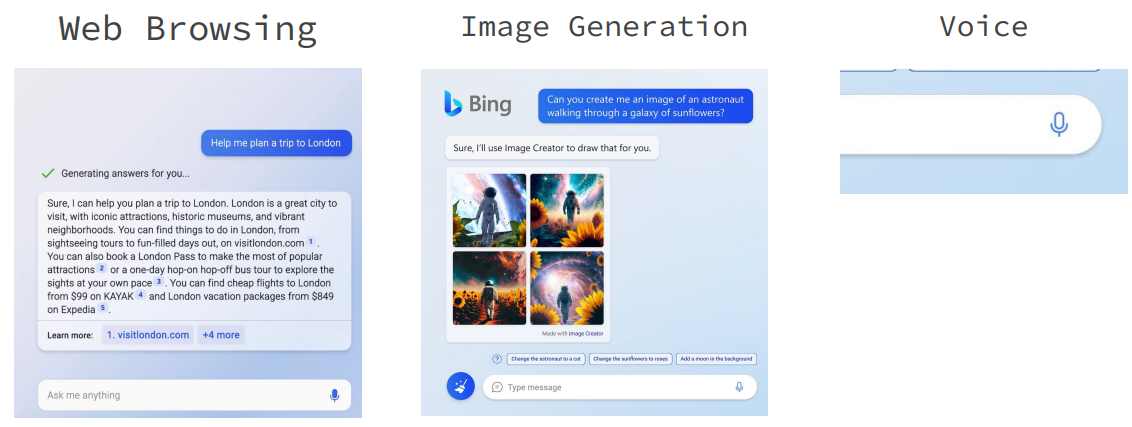
\includegraphics[width=\linewidth,keepaspectratio]{promptengg93}

		{\tiny (Ref: The Complete Prompt Engineering for AI Bootcamp (2023))}
		\end{center}	

\end{frame}

%%%%%%%%%%%%%%%%%%%%%%%%%%%%%%%%%%%%%%%%%%%%%%%%%%%%%%%%%%%
\begin{frame}[fragile]\frametitle{Microsoft Bing (GPT 4) Use Cases}


		\begin{center}
		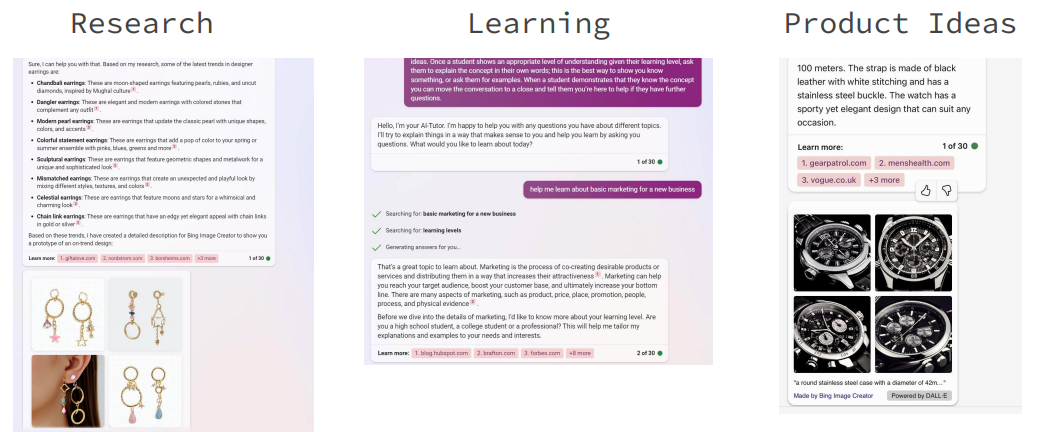
\includegraphics[width=\linewidth,keepaspectratio]{promptengg94}

		{\tiny (Ref: The Complete Prompt Engineering for AI Bootcamp (2023))}
		\end{center}	

\end{frame}



%%%%%%%%%%%%%%%%%%%%%%%%%%%%%%%%%%%%%%%%%%%%%%%%%%%%%%%%%%%
\begin{frame}[fragile]\frametitle{Falcon}


\begin{columns}
    \begin{column}[T]{0.6\linewidth}
		\begin{center}
		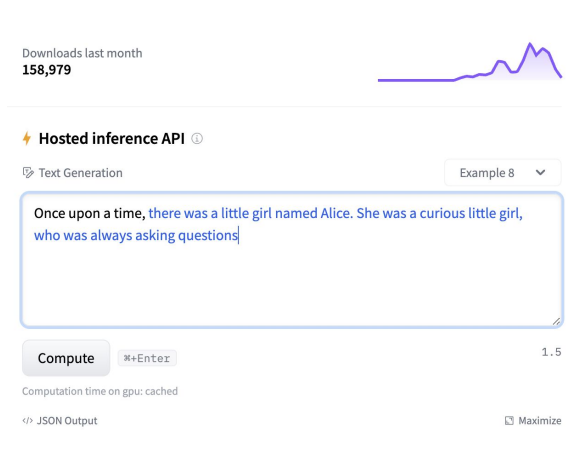
\includegraphics[width=\linewidth,keepaspectratio]{promptengg95}

		{\tiny (Ref: The Complete Prompt Engineering for AI Bootcamp (2023))}
		\end{center}	
    \end{column}
    \begin{column}[T]{0.4\linewidth}
		Access it via HuggingFace transformers library https://share.descript.com/view/Qp6mcWh3V2a
		7B and 40B models as well as instruct fine-tuned
    \end{column}
  \end{columns}
\end{frame}


%%%%%%%%%%%%%%%%%%%%%%%%%%%%%%%%%%%%%%%%%%%%%%%%%%%%%%%%%%%
\begin{frame}[fragile]\frametitle{Falcon Features}

\begin{itemize}
\item Free for commercial use
\item Open source
\item Possible to fine-tune
\end{itemize}	 

\end{frame}

%%%%%%%%%%%%%%%%%%%%%%%%%%%%%%%%%%%%%%%%%%%%%%%%%%%%%%%%%%%
\begin{frame}[fragile]\frametitle{Falcon Use Cases}


		\begin{center}
		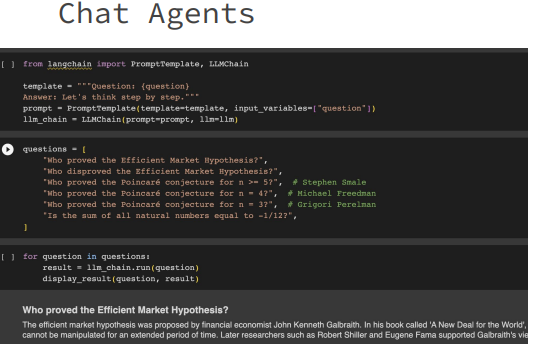
\includegraphics[width=0.5\linewidth,keepaspectratio]{promptengg96}

		{\tiny (Ref: The Complete Prompt Engineering for AI Bootcamp (2023))}
		\end{center}	

\end{frame}









%%%%%%%%%%%%%%%%%%%%%%%%%%%%%%%%%%%%%%%%%%%%%%%%%%%%%%%%%%%
\begin{frame}[fragile]\frametitle{Leader board (May 2023)}


		\begin{center}
		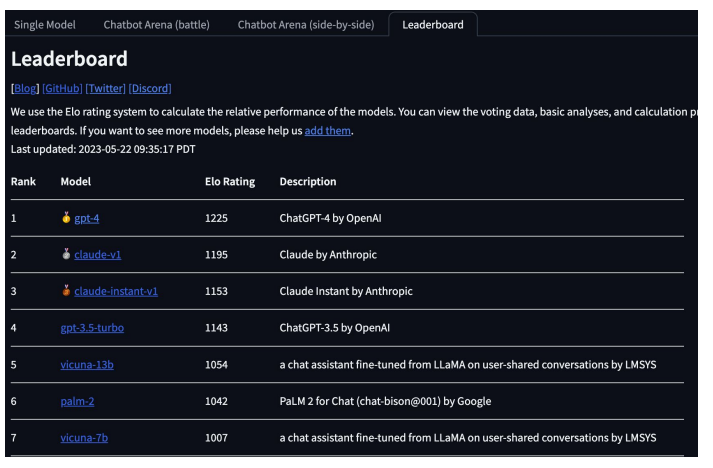
\includegraphics[width=\linewidth,keepaspectratio]{promptengg89}

		{\tiny (Ref: The Complete Prompt Engineering for AI Bootcamp (2023))}
		\end{center}	

\end{frame}